\subsubsection{Data Labelling Techniques}

\begin{method} \hlt{Labelling with Fixed-Time Horizon Method}\\
Given features matrix $X$ with $I$ rows, $\{X_i\}_{i = 1, \ldots, I}$ drawn from some bards with index $t = 1, \ldots, T$, where $I \leq T$, let an observation $X_i$ be assigned a label $y_i \in \{-1, 0, 1\}$,
\begin{align}
y_i &=
\begin{cases}
-1 \ \ \ \text{if } r_{t_{i,0}, t_{i,0} + h} < -\tau \\
0 \ \ \ \ \ \ \text{if } \abs{r_{t_{i,0}, t_{i,0} + h}} \leq \tau \\
1 \ \ \ \ \ \ \text{if } r_{t_{i,0}, t_{i,0} + h} > \tau
\end{cases} \nonumber \\
r_{t_{i,0}, t_{i,0} + h} &= \frac{p_{t_{i,0}+h}}{p_{t_{i,0}}} - 1 \nonumber
\end{align}
where $\tau$ is a pre-defined constant threshold, $t_{i,0}$ is index of bar immediately after $X_i$ takes place, $t_{i,0} + h$ is index of $h$-th bar after $t_{i,0}$, and $r_{t_{i,0}, t_{i,0} + h}$ is price return over bar horizon $h$.
\end{method}

\begin{remark} \hlt{Limitations of Fixed-Time Horizon Method}
\begin{enumerate}[label=\roman*.]
\setlength{\itemsep}{0pt}
\item Time bars do not exhibit good statistical properties (as seen earlier)
\item The same threshold $\tau$ is applied regardless of observed volatility.\\
Compute daily volatility at intraday estimation points, applying span of $n$ days t an exponentially weighted moving standard deviation.
\end{enumerate}
\end{remark}

\begin{method} \hlt{Labelling with Triple-Barrier Method}\\
Labels an observation according to first barrier touched out of three barriers.
\begin{enumerate}[label=\roman*.]
\setlength{\itemsep}{0pt}
\item Set two horizontal barriers and one vertical barrier. Horizontal barriers are defined by profit-taking and stop-loss limits, which are a dynamic function of estimated volatility (realised or implied). Third barrier is the number of bars elapsed since the position was taken (expiration limit).
\item If upper barrier is touched first, label observation as $1$. If lower barrier is touched first, label observation as $-1$. If vertical barrier is touched first, either label by sign of the return or with $0$.
\end{enumerate}
Note that the method is path-dependent. To label an observation, need to account for entire path spanning $[t_{i,0}, t_{i,0} + h]$ where $h$ defines the vertical barrier (expiration limit). Let $t_{i,1}$ be the time of first barrier touch with return as $r_{t_{i,0}, t_{i,1}}$. The horizontal barriers may not be symmetric.
\end{method}

\begin{remark} \hlt{Triple-Barrier Method Configurations}\\
Denote a barrier configuration by triplet $[pt, sl, t1]$ which are the upper barrier, lower barrier, physical barrier. Set value as $0$ if barrier is inactive, and $1$ if barrier is active.\\
The three useful configurations are:
\begin{enumerate}[label=\roman*.]
\setlength{\itemsep}{0pt}
\item $[1,1,1]$: to realise profit, but have set a maximum tolerance for losses and a holding period.
\item $[0,1,1]$: to exit after a number of bars, unless stopped-out.
\item $[1,1,0]$: take profit as long as not stopped-out.
\end{enumerate}
The three less realistic configurations are:
\begin{enumerate}[label=\roman*.]
\setlength{\itemsep}{0pt}
\item $[0,0,1]$: equivalent to fixed-time horizon method. 
\item $[1,0,1]$: position held until a profit is made or maximum holding period is exceeded, without regard for immediate unrealised losses
\item $[1,0,0]$: position is held until a profit is made. Could lock in loose position for years.
\end{enumerate}
The two illogical configurations are:
\begin{enumerate}[label=\roman*.]
\setlength{\itemsep}{0pt}
\item $[0,1,0]$: aimless. Hold position until stopped-out.
\item $[0,0,0]$: no barriers. Position locked forever, no label generated.
\end{enumerate}
\end{remark}

\begin{figure}[H]
\centering
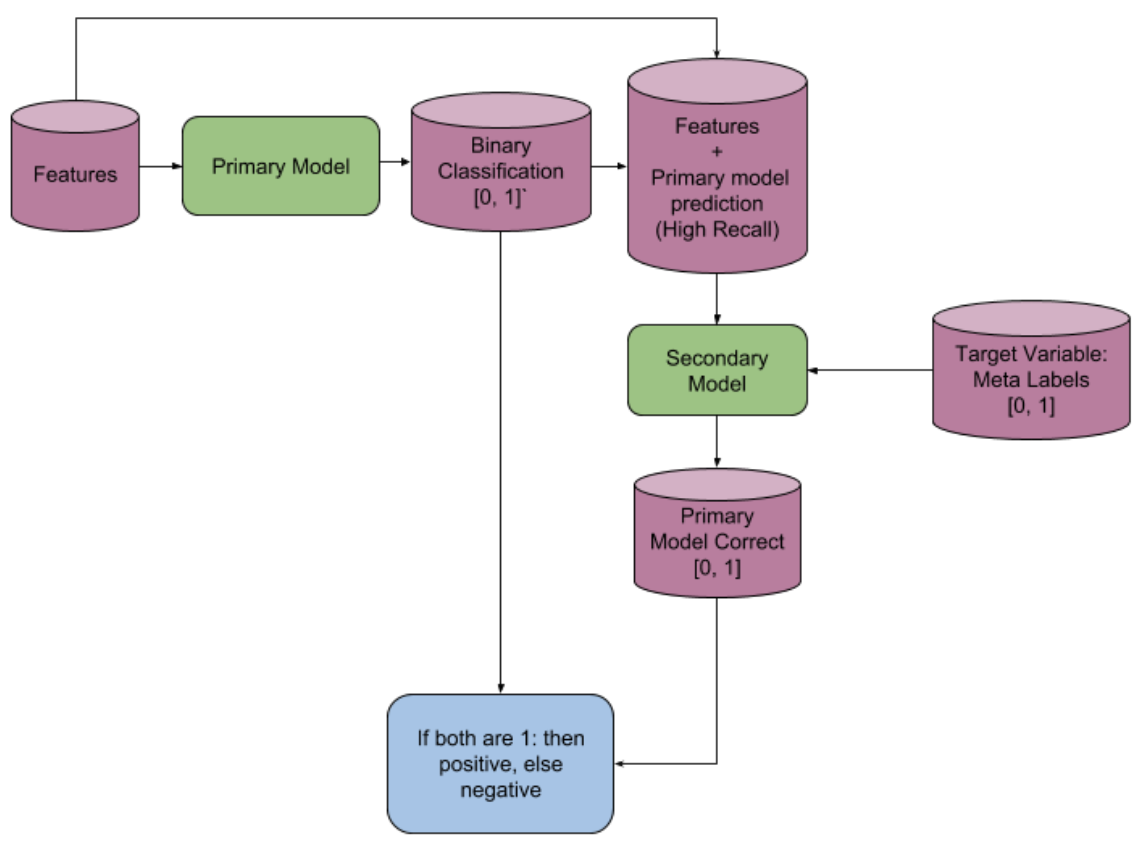
\includegraphics[scale=0.4]{/intro/metalabel}
\caption{Meta-Labelling Process}
\end{figure}

\begin{method} \hlt{Meta-Labelling}\\
The technique is particularly helpful to achieve higher F1-scores.\\
First, build a model that achieves high recall, even if precision is not particularly high. Second, correct for low precision by applying meta-labelling to positives predicted by primary model.\\
Meta-labelling will filter out false positives, where majority of positives have been identified by primary model. The second model's purpose is to determine if the positive from primary model is true or false.
\begin{enumerate}[label=\roman*.]
\setlength{\itemsep}{0pt}
\item Train a primary model (binary classification)
\item A threshold level is determined at which the primary model has a high recall, ROC curves could be used to help determine a good level.
\item Typical features of second model are as follows:
\begin{enumerate}[label=\roman*.]
\setlength{\itemsep}{0pt}
\item Primary model features concatenated with predictions from first model.
\item Market state
\item Features indicative of false positives
\item Distribution related
\item Recent model performance
\end{enumerate}
Meta Labels are used as target variable in second model. Fit the second model
\item Prediction from the secondary model is combined with the prediction from the primary model and only where both are true, is your final prediction true.
\end{enumerate}
\end{method}

\begin{remark} \hlt{Limitations of Meta-Labelling}
\begin{enumerate}[label=\roman*.]
\setlength{\itemsep}{0pt}
\item If model has overfit the data, meta-labelling will not add much value
\item If every trade is not treated as an independent observation, the meta-model is forced to determine day-to-day exposures, which is the wrong way to apply the technique
\item Technique trades recall for precision. Require a large number of trades to train on, while being happy with reduction in trade frequency
\end{enumerate}
\end{remark}

